%%%%%%%%%%%%%%%%%%%%%%% file template.tex %%%%%%%%%%%%%%%%%%%%%%%%%
%
% This is a general template file for the LaTeX package SVJour3
% for Springer journals.          Springer Heidelberg 2010/09/16
%
% Copy it to a new file with a new name and use it as the basis
% for your article. Delete % signs as needed.
%
% This template includes a few options for different layouts and
% content for various journals. Please consult a previous issue of
% your journal as needed.
%
%%%%%%%%%%%%%%%%%%%%%%%%%%%%%%%%%%%%%%%%%%%%%%%%%%%%%%%%%%%%%%%%%%%
%
% First comes an example EPS file -- just ignore it and
% proceed on the \documentclass line
% your LaTeX will extract the file if required
\begin{filecontents*}{example.eps}
%!PS-Adobe-3.0 EPSF-3.0
%%BoundingBox: 19 19 221 221
%%CreationDate: Mon Sep 29 1997
%%Creator: programmed by hand (JK)
%%EndComments
gsave
newpath
  20 20 moveto
  20 220 lineto
  220 220 lineto
  220 20 lineto
closepath
2 setlinewidth
gsave
  .4 setgray fill
grestore
stroke
grestore
\end{filecontents*}
%
\RequirePackage{fix-cm}
%
%\documentclass{svjour3}                     % onecolumn (standard format)
%\documentclass[smallcondensed]{svjour3}     % onecolumn (ditto)
\documentclass[smallextended]{svjour3}       % onecolumn (second format)
%\documentclass[twocolumn]{svjour3}          % twocolumn
%
\smartqed  % flush right qed marks, e.g. at end of proof
%
\usepackage{graphicx}
\usepackage{amsmath}
%
% \usepackage{mathptmx}      % use Times fonts if available on your TeX system
%
% insert here the call for the packages your document requires
%\usepackage{latexsym}
% etc.
%
% please place your own definitions here and don't use \def but
% \newcommand{}{}
%
% Insert the name of "your journal" with
% \journalname{myjournal}
%
\begin{document}

\title{Comparison of Mixed Integer Programming Formulations for the Shared Multicast Tree Problem%\thanks{Grants or other notes
%about the article that should go on the front page should be
%placed here. General acknowledgments should be placed at the end of the article.}
}
\subtitle{Tightening the LP bounds}

%\titlerunning{Short form of title}        % if too long for running head

\author{Dag Haugland        \and
        Marika Ivanova %etc.
}

%\authorrunning{Short form of author list} % if too long for running head

\institute{F. Author \at
              first address \\
              Tel.: +123-45-678910\\
              Fax: +123-45-678910\\
              \email{fauthor@example.com}           %  \\
%             \emph{Present address:} of F. Author  %  if needed
           \and
           S. Author \at
              second address
}

\date{Received: date / Accepted: date}
% The correct dates will be entered by the editor


\maketitle

\begin{abstract}
Insert your abstract here. Include keywords, PACS and mathematical
subject classification numbers as needed.
\keywords{First keyword \and Second keyword \and More}
% \PACS{PACS code1 \and PACS code2 \and more}
% \subclass{MSC code1 \and MSC code2 \and more}
\end{abstract}

\section{Introduction}

\label{intro}

The purpose of a multicast communication in a wireless ad-hoc network is to route information from a sending device to a set of receiving devices. Given a set of wireless devices and distances between them, the task is to assign power to each device, so that the demands of the communication are met and the energy consumption is as low as possible, assuming their locations are fixed. Power efficiency is an important measure in designing ad-hoc wireless networks since the devices typically use batteries as power supply and are therefore heavily energy-constrained. Individual devices work as transceivers, which means that they have the ability to both transmit and receive a signal. Moreover, the power level of a device can be dynamically adjusted during a multicast session.

Unlike wired networks, nodes in ad-hoc wireless networks use omnidirectional antennas, and hence a message reaches all nodes within the communication range of the sender. This range is determined by the power assigned to the sender, which is the maximum rather than the sum of the powers necessary to reach all intended receivers. This feature is often referred to as the wireless multicast advantage \cite{Wieseltier00onthe}. 

\subsection{Related work}
\subsection{Definitions and notation}
An ad-hoc wireless network is modelled by a complete graph $G=(V,E)$
\section{MIP Formulations}
\label{sec:1}
In this section, we state the known MIP formulation of the shared multicast tree problem and relations between them. Several strengthening valid inequalities are also presented.
\subsection{Original SMT Model}
The first model we consider is slightly improved SMT model introduced in \ref{ref:ivanova}, which contains a weaker version of constrainte (\ref{}). This model extends the SBT formulation from \ref{ref:haugland} by the Steiner nodes in order to formulate the multicast version of the problem. The model uses three sets of variables defined as follows:
\newline\newline
  $z_{ij}=
	\begin{cases}
    1 & \text{if edge $\{i,j\} \in E$ is in the solution},\\
    0 & \text{otherwise},
  \end{cases}$
\newline\newline
  $x^{s}_{ij}=
	\begin{cases}
    1 & \text{if arc $(i,j) \in A$ is used to transmit a message from $s\in D$},\\
    0 & \text{otherwise}.
  \end{cases}$
  \newline\newline
  $y^s_{ij}=
	\begin{cases}
    1 & \text{if node $i \in V$ uses power $p_{ij}$ to transmit a message from $s\in D$},\\
    0 & \text{otherwise}.
  \end{cases}$
\newline
\newline    
\begin{subequations}
\begin{flalign}
\label{objective:dd} &\makebox[0pt][l]{$\displaystyle{}\min \sum\limits_{(i,j) \in A} \sum\limits_{s \in D} p_{ij} y^s_{ij} $}  & &&\\ \notag  
\text{s.t.}&  &  &                 && \\	\
\label{con:dd:maxsize}\sum\limits_{\{i,j\}\in E}z_{ij} & \leq  N-1 &  && \\
\label{con:dd:arrowFromDest} \sum\limits_{j\in V_i}x^s_{ji} & = 1 && i,s\in D,i\neq s && \\ 
\label{con:dd:arrowFromNonDestB} \sum\limits_{j\in V_{i}}x^s_{ji} & \leq 1 && i\in V \setminus D, s\in D   &&\\	
\label{con:dd:arrowFromNonDestA} x^s_{ik}  & \leq \sum\limits_{j\in V_{i}\setminus \{k\}}x^s_{ji} && i\in V \setminus D,(i,k)\in A, s\in D   &&\\	
\label{con:dd:extraCon} \sum\limits_{j\in V_{i}}x^s_{ji} & \leq \sum\limits_{j\in V_{i}}x^s_{ij} &&  	i\in V\setminus D, s\in D  &&\\	
\label{con:dd:oneDir} x^s_{ij} + x^s_{ji} & = z_{ij} && \{i,j\}\in E, s\in D &&\\
\label{con:dd:startInSource}  x^i_{ji}    & = 0   &&  i\in D, (j,i)\in A &&\\		 
\label{con:dd:yvar} x^s_{ij} & \leq \sum\limits_{k\in V:p_{ik}\geq p_{ij}}y^s_{ik} && s\in D, (i,j)\in A &&\\  
& \label{con:dd:vardim}	\mathbf{z} \in \{0,1\}^{E}, \mathbf{x},\mathbf{y}\in \{0,1\}^{A\times D} &&	
\end{flalign}~
\end{subequations}   
Let $(\mathbf{x},\mathbf{y}, \mathbf{z})$ be an optimal solution to the SMT model above. Then, the vector $\mathbf{x^s}\in \{0,1\}^{A}$ encapsulates broadcast Steiner arborescences for a source $s\in D$. From $\mathbf{z}\in \{0,1\}^E$ we obtain the resulting (undirected) broadcast Steiner tree. Finally, $\mathbf{y^s}\in \{0,1\}^{A}$ describes the links determining the power levels. The graph induced by $\mathbf{y}$ is  a subgraph of the tree induced by $\mathbf{x}$, and is not necessarily connected.

The number of edges in the resulting Steiner tree is constrained by (\ref{con:dd:maxsize}). Imposing a lower bound $M-1$ on the size of the spanning tree would neither reduce the space of feasible solutions nor increase the strength of the model. If the tree does not contain any Steiner nodes, its size is the lower bound, while if all nodes are used (either as Steiner nodes, or $D = V$), its size equals the upper bound. Constraints (\ref{con:dd:arrowFromDest}) ensures that a message from source $s$ reaches a destination $i$ from exactly one neighbour $j\in V_i$. Analogously, (\ref{con:dd:arrowFromNonDestB}) covers the case when $j \in V\setminus D$: For every source $s$, there is at most one inbound arc to a non-destination $i$. 

If a non-destination $i$ forwards a message from $s$ towards $k$, the message must come from exactly one neighbour $j$ different from $k$, because there is no point in sending the signal backwards. This is ensured by constraint (\ref{con:dd:arrowFromNonDestA}). Note that assuming there is no outgoing arc from a non-destination $j$, (\ref{con:dd:arrowFromNonDestA}) does not prevent $j$ from being a leaf in $G_{\mathbf{x^s}}$. We make such undesired solutions impossible by adding constraint (\ref{con:dd:extraCon}) reducing the set of feasible solutions. However, (\ref{con:dd:extraCon}) is not necessary, because a solution, where a non-destination that does not relay any message is assigned a non-zero power, would be filtered out by optimality. The expression (\ref{con:dd:oneDir}) enforces that an edge $\{i,j\}$ is a part of a solution if and only if for every $s\in D$, either $(i,j)$ or $(i,j)$ is an arc used for sending a message from $s$. The next constraint (\ref{con:dd:startInSource}) expresses that a transmission initiated by $s\in D$ cannot reach $s$ again, which implies non-existence of a directed cycle containing $s$. Finally, by (\ref{con:dd:yvar}), we define a relation between $x$-variables and $y$-variables. When arc $(i,j)$ is used for transmission of a message from $s\in D$, vertex $i$ relaying the message must be assigned power at least $p_{ij}$.
\subsection{$s,t$-Flow Extension}
Consider a network flow problem where one unit of flow must be sent between every pair  $(s,t)$ of destinations. In order to model this requirements, we introduce a variable $f^{st}_{ij}$ as follows:
\newline\newline
  $f_{ij}^{st}=
	\begin{cases}
    1 & \text{if arc $\{i,j\} \in A$ carries 1 unit of flow from $s\in D$ to $t\in D$},\\
    0 & \text{otherwise}.
  \end{cases}$
\newline\newline

The original SMT formulation can be extended and strengthened by flow constraints for each $(s,t)$-pair.
\newline
\newline    
\begin{subequations}
\begin{flalign}
\label{objective:dd} \makebox[0pt][l]{$\displaystyle{} \min \sum\limits_{(i,j) \in A} \sum\limits_{s \in D} p_{ij} y^s_{ij} $}  \\ 
\text{s.t.}    \notag   \\	
(\ref{objective:dd}),\dots,(\ref{con:dd:yvar}) \notag \\ 
 \label{con:mf:flowNormal}  \sum\limits_{\substack{ j\in V_i}}f^{st}_{ij}-\sum\limits_{\substack{j\in V_i }}f^{st}_{ji}    & = 0   \quad \quad\quad 			  i\in V\setminus\{s,t\}, s,t\in D, s \neq t &\\	
\label{con:mf:flowDest}  \sum\limits_{\substack{ j\in V_t }}f^{st}_{tj}-\sum\limits_{\substack{j\in V_t}}f^{st}_{jt}    & = -1  \quad\quad ~ s,t\in D, s \neq t &\\	
 \label{con:mf:fcap}   f^{st}_{ij} &\leq  x^{s}_{ij},\quad\quad    (i,j)\in A,  s,t\in D, s \neq t  & \\ 		 			 	 
 \label{con:mf:fsym}   f^{st}_{ij} &=  f^{ts}_{ji},  \quad\quad(i,j)\in A,  s,t\in D, s \neq t  &\\   	
\label{con:mf:xydim}	\mathbf{z} \in \{0,1\}^{E}, \mathbf{x},\mathbf{y}\in \{0,1\}^{A\times D}, & \mathbf{f}\in\{0,1\}^{A\times D\times D}. 
\end{flalign}~
\end{subequations}  
The flow conservation constraints (\ref{con:mf:flowNormal})-(\ref{con:mf:flowDest}) guarantee that for each $s,t\in D$ there is a flow of one unit from $s$ to $t$. Next constraint (\ref{con:mf:fcap}) expresses that if an arc $(i,j)$ carries an $s,t$-flow , then this arc is used for sending a message initiated in $s$. The flow symmetry (\ref{con:mf:fsym}) states that arc $(i,j)$ carries a flow from $s$ to $t$ if and only if arc $(j,i)$ carries a flow from $t$ to $s$.

This model can be further extended by valid inequalities strengthening LP bounds
  \begin{subequations}
  \begin{flalign}
\label{con:vi:xImpY}  x^{s}_{ij} & \leq \sum\limits_{t\in D\setminus\{s\}}  f^{st}_{ij},  \quad\quad    (i,j)\in A,s\in D \\
 \label{con:vi:Y1}  \sum\limits_{j\in V\setminus\{s\}}  y^{s}_{sj} & =1,  \quad\quad\quad\quad\quad\quad    s\in D \\
\label{con:vi:f2dest}  f^{st_1}_{ij}-f^{st_2}_{ij}+f^{t_1t_2}_{ij} & \geq 0, \quad\quad\quad\quad\quad\quad i,j \in V,s,t_1,t_2\in D, \\
   &     \notag\quad\quad\quad\quad\quad\quad\quad\quad i\neq j, s\neq t_1,s\neq t_2, t_1\neq t_2  \\
\label{con:vi:sumYImpSumX} \sum\limits_{i\in V\setminus\{j\} }y^{s}_{ji} & \geq \sum\limits_{i\in V\setminus\{j\}}  x^{s}_{ij},   \quad\quad   j\in V\setminus D, s\in D \\
\label{con:vi:sumFImpSumY} \sum\limits_{i\in V\setminus\{j\}, p_{ji}\geq p_{jk}  }f^{st}_{ji} & \leq \sum\limits_{i\in V\setminus\{j\}, p_{ji}\geq p_{jk}}  y^{s}_{ji},   j\in V, s, t\in D, s \neq t, k\in V                     
                      \end{flalign}
  \end{subequations}
\subsection{SMT based on Polzin's Minimum Steiner Tree formulation}

There are many formulations for the Steiner minimum tree problem, that can be a basis for our SMT problem. We consider the formulation $P_{F^2}$, the strongest model studied in \cite{polzin}. The model contains variables
%\newline
%  $y^s_{ij}=
%	\begin{cases}
%    1 & \text{if node $i \in V$ uses power $p_{ij}$ to transmit messages from $s\in D$},\\
%    0 & \text{otherwise}.
%  \end{cases}$
\newline\newline  
  $\check{f}^{st}_{ij}=
	\begin{cases}
    1 & \text{if arc $(i,j) \in A$ carries a flow from the source to both $s,t\in D_1$},\\
    0 & \text{otherwise}.
  \end{cases}$
\newline\newline  
  $f^{t}_{ij}=
	\begin{cases}
    1 & \text{if arc $(i,j) \in A$ carries a flow from the source to $t\in D_1$},\\
    0 & \text{otherwise}.
  \end{cases}$  
\newline\newline  
  $x_{ij}=
	\begin{cases}
    1 & \text{if arc $(i,j) \in A$ is in the solution},\\
    0 & \text{otherwise}.
  \end{cases}$  
\newline
\newline   
The $x$-variables encapsulating the resulting tree correspond to arcs, while analogous $z$-variables in $s,t$-flow model correspond to edges. Hence, a solution obtained by $s,t$-flow is an undirected tree, while $P_{F^2}$ produces an arborescence.
\subsection{Relation between SMT a PF2}
\section{Experimental Evaluation}

The practical part of this work focuses on comparison of the models presented in the previous section. As the main focus of this study is to determine tighter bounds, the conducted experiments are designed for this purpose. 

\subsection{Constraint generation}
The stronger SMT models are too large and are therefore not very practical as computation of rather smaller instances takes prohibitively long time. That is also the case of the model SMT-MF. The main idea of how to make this model more useful in practice is to dynamically add only those flow constraints that are violated. First, we relax the flow constraints which means that we solve only the LP relaxation of the original SMT model. This gives the vector $\mathbf{x}$, which, by constraint (\ref{smtmf:cap}), acts as a capacity vector, and determines the maximum possible value of a flow through certain arc. Next, we go through all possible $s-t$ pairs of destinations and check whether the flow constraints are fulfilled for the particular $s$ and $t$. New flow constraints for some (possibly all) $s-t$ pairs that violate flow constraints are added to the model and the whole process is repeated until there are no violated flow constraints for any $s-t$ pair. The algorithm \ref{alg:congen} describes this process formally.


There are various strategies how to determine which violated flow constraints will be added to the model. 

\section{Conclusion and Future Work}
\label{sec:2}
as required. Don't forget to give each section
and subsection a unique label (see Sect.~\ref{sec:1}).
\paragraph{Paragraph headings} Use paragraph headings as needed.
\begin{equation}
a^2+b^2=c^2
\end{equation}

% For one-column wide figures use
\begin{figure}
% Use the relevant command to insert your figure file.
% For example, with the graphicx package use
  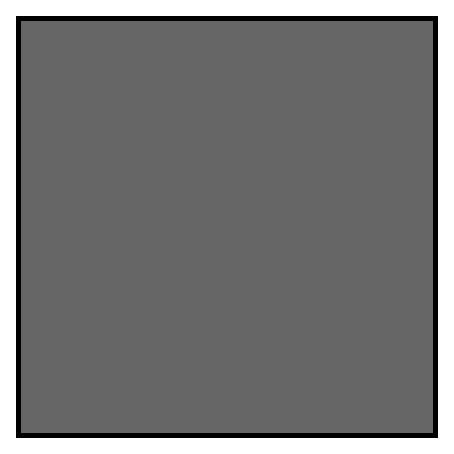
\includegraphics{example.eps}
% figure caption is below the figure
\caption{Please write your figure caption here}
\label{fig:1}       % Give a unique label
\end{figure}
%
% For two-column wide figures use
\begin{figure*}
% Use the relevant command to insert your figure file.
% For example, with the graphicx package use
  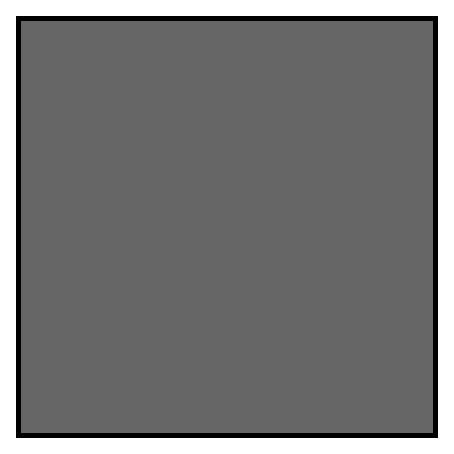
\includegraphics[width=0.75\textwidth]{example.eps}
% figure caption is below the figure
\caption{Please write your figure caption here}
\label{fig:2}       % Give a unique label
\end{figure*}
%
% For tables use
\begin{table}
% table caption is above the table
\caption{Please write your table caption here}
\label{tab:1}       % Give a unique label
% For LaTeX tables use
\begin{tabular}{lll}
\hline\noalign{\smallskip}
first & second & third  \\
\noalign{\smallskip}\hline\noalign{\smallskip}
number & number & number \\
number & number & number \\
\noalign{\smallskip}\hline
\end{tabular}
\end{table}


%\begin{acknowledgements}
%If you'd like to thank anyone, place your comments here
%and remove the percent signs.
%\end{acknowledgements}

% BibTeX users please use one of
%\bibliographystyle{spbasic}      % basic style, author-year citations
%\bibliographystyle{spmpsci}      % mathematics and physical sciences
%\bibliographystyle{spphys}       % APS-like style for physics
%\bibliography{}   % name your BibTeX data base

% Non-BibTeX users please use
\begin{thebibliography}{}
%
% and use \bibitem to create references. Consult the Instructions
% for authors for reference list style.
%
\bibitem{RefJ}
% Format for Journal Reference
Author, Article title, Journal, Volume, page numbers (year)
% Format for books
\bibitem{RefB}
Author, Book title, page numbers. Publisher, place (year)
% etc
\end{thebibliography}

\end{document}
% end of file template.tex

